% ================= Appendix A =================
\chapter{Raw Dataset}
\label{app:A.1}
 \label{fig:samplerawdatas}
\begin{figure}[H]
    \centering
    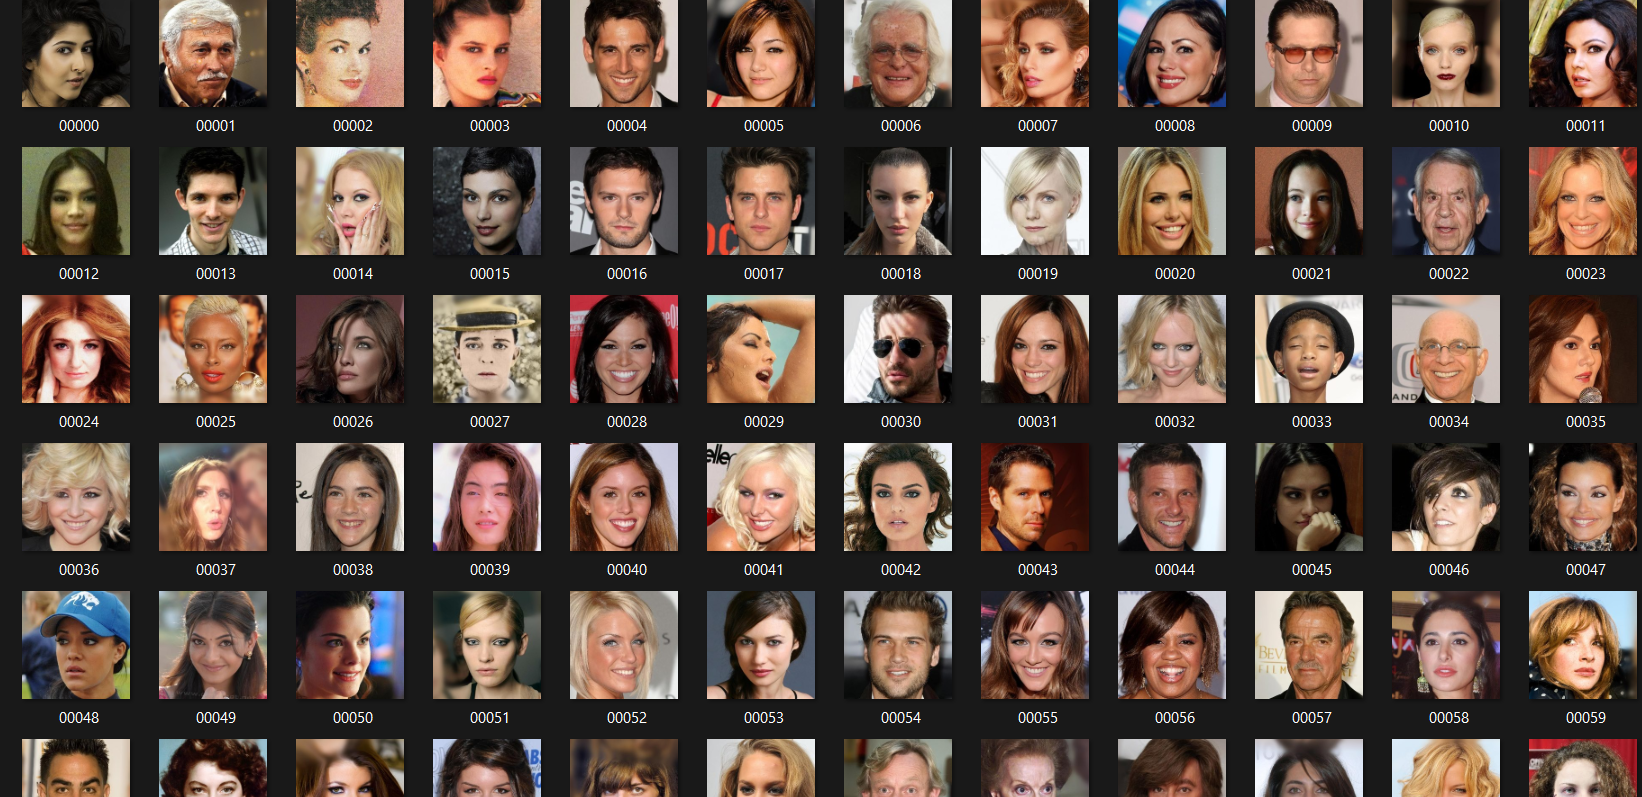
\includegraphics[width=0.75\textwidth]{img/raw_dataset.png}
    \caption{Sample raw dataset}
   
\end{figure}



% ================= Appendix B =================
\chapter{Data Processed}
\label{app:B1}

\section{Data1}
\begin{figure}[H]
    \centering
    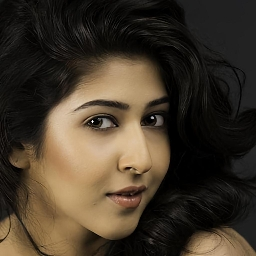
\includegraphics[width=0.5\textwidth]{img/d1.jpeg}
    \caption{Main interface}
\end{figure}

\section{Data1 Landmark}
\begin{figure}[H]
    \centering
    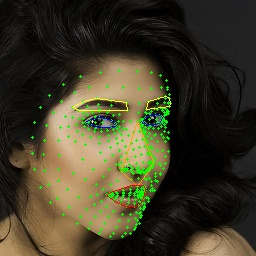
\includegraphics[width=0.5\textwidth]{img/d2.jpeg}
    \caption{Input Image}
\end{figure}

\section{Semantic Masks}

\begin{figure}[H]
\centering

% Row 1
\begin{minipage}{0.48\textwidth}
    \centering
    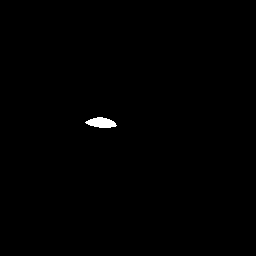
\includegraphics[width=0.65\linewidth]{img/2/00000_semantic_left_eye.png}
    \caption{Semantic mask for the left eye region}
    \label{fig:semantic_left_eye}
\end{minipage}
\hfill
\begin{minipage}{0.48\textwidth}
    \centering
    
\includegraphics[width=0.65\linewidth]{img/2/00000_semantic_left_eyebrow.png}
    \caption{Semantic mask for the left eyebrow region}
    \label{fig:semantic_left_eyebrow}
\end{minipage}

\vspace{0.3cm}

% Row 2
\begin{minipage}{0.48\textwidth}
    \centering
    
\includegraphics[width=0.65\linewidth]{img/2/00000_semantic_mouth.png}
    \caption{Semantic mask for the mouth region}
    \label{fig:semantic_mouth}
\end{minipage}
\hfill
\begin{minipage}{0.48\textwidth}
    \centering
    
\includegraphics[width=0.65\linewidth]{img/2/00000_semantic_nose.png}
    \caption{Semantic mask for the nose region}
    \label{fig:semantic_nose}
\end{minipage}

\vspace{0.3cm}

% Row 3
\begin{minipage}{0.48\textwidth}
    \centering
    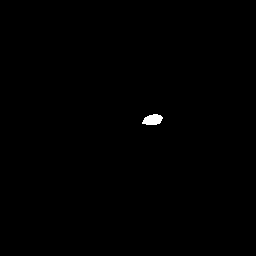
\includegraphics[width=0.65\linewidth]{img/2/00000_semantic_right_eye.png}
    \caption{Semantic mask for the right eye region}
    \label{fig:semantic_right_eye}
\end{minipage}
\hfill
\begin{minipage}{0.48\textwidth}
    \centering
    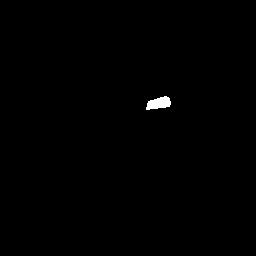
\includegraphics[width=0.65\linewidth]{img/2/00000_semantic_right_eyebrow.png}
    \caption{Semantic mask for the right eyebrow region}
    \label{fig:semantic_right_eyebrow}
\end{minipage}

\end{figure}

\clearpage

\section{Heatmaps}

\begin{figure}[H]
\centering

% Row 1
\begin{minipage}{0.48\textwidth}
    \centering
    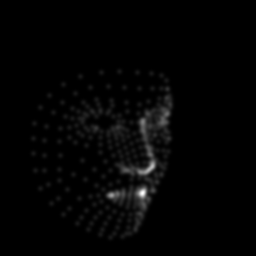
\includegraphics[width=0.65\linewidth]{img/1/1_00000_semantic_left_eye.png}
    \caption{Landmark heatmap for the left eye region}
    \label{fig:heatmap_left_eye}
\end{minipage}
\hfill
\begin{minipage}{0.48\textwidth}
    \centering
    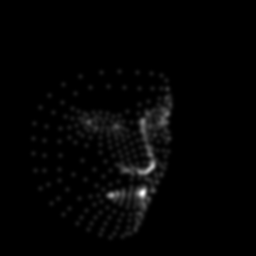
\includegraphics[width=0.65\linewidth]{img/1/1_00000_semantic_left_eyebrow.png}
    \caption{Landmark heatmap for the left eyebrow region}
    \label{fig:heatmap_left_eyebrow}
\end{minipage}

\vspace{0.3cm}

% Row 2
\begin{minipage}{0.48\textwidth}
    \centering
    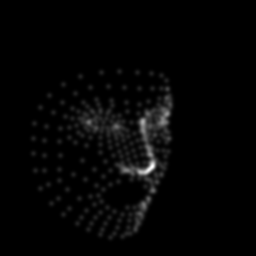
\includegraphics[width=0.65\linewidth]{img/1/1_00000_semantic_mouth.png}
    \caption{Landmark heatmap for the mouth region}
    \label{fig:heatmap_mouth}
\end{minipage}
\hfill
\begin{minipage}{0.48\textwidth}
    \centering
    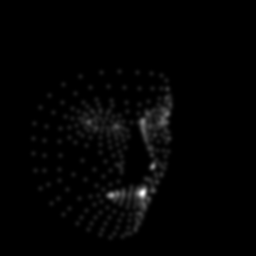
\includegraphics[width=0.65\linewidth]{img/1/1_00000_semantic_nose.png}
    \caption{Landmark heatmap for the nose region}
    \label{fig:heatmap_nose}
\end{minipage}

\vspace{0.3cm}

% Row 3
\begin{minipage}{0.48\textwidth}
    \centering
    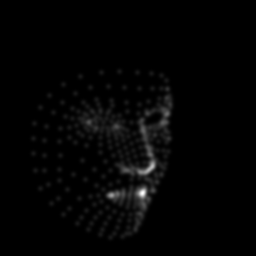
\includegraphics[width=0.65\linewidth]{img/1/1_00000_semantic_right_eye.png}
    \caption{Landmark heatmap for the right eye region}
    \label{fig:heatmap_right_eye}
\end{minipage}
\hfill
\begin{minipage}{0.48\textwidth}
    \centering
    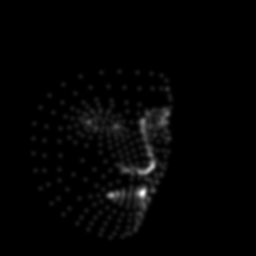
\includegraphics[width=0.65\linewidth]{img/1/1_00000_semantic_right_eyebrow.png}
    \caption{Landmark heatmap for the right eyebrow region}
    \label{fig:heatmap_right_eyebrow}
\end{minipage}

\end{figure}


% ================= Appendix C =================
\chapter{Image Pre-processing Pipeline Details}
\label{app:preprocessing}
\section{Original Input (256*256)}
\label{app:C1}
\begin{figure}[H]
    \centering
    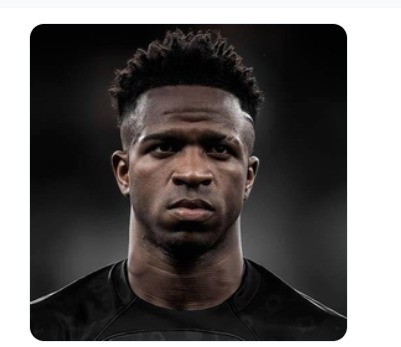
\includegraphics[width=0.5\textwidth]{img/b1.jpeg}
    \caption{Original Input (256*256)}
\end{figure}

\section{Landmarks Detection}
\label{app:C2}
\begin{figure}[H]
    \centering
    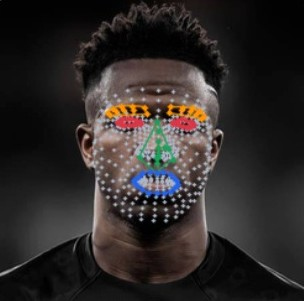
\includegraphics[width=0.5\textwidth]{img/b2.jpeg}
    \caption{Landmarks Detection}
\end{figure}

\section{Masked Input}
\label{app:C3}
\begin{figure}[H]
    \centering
    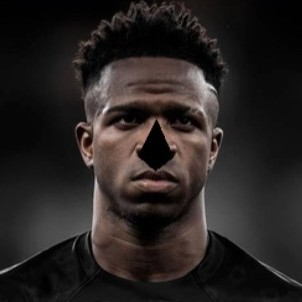
\includegraphics[width=0.5\textwidth]{img/b3.jpeg}
    \caption{Masked Input}
\end{figure}

\section{Binary Mask}
\label{app:C4}
\begin{figure}[H]
    \centering
    
\includegraphics[width=0.5\textwidth]{img/b4.jpeg}
    \caption{Binary Mask}
\end{figure}

\section{Landmark Heatmap}
\label{app:C5}
\begin{figure}[H]
    \centering
    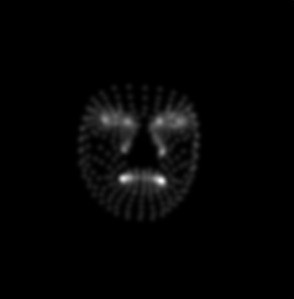
\includegraphics[width=0.5\textwidth]{img/b5.jpeg}
    \caption{Landmark Heatmap}
\end{figure}

\section{Raw Generator Output}
\label{app:C6}
\begin{figure}[H]
    \centering
    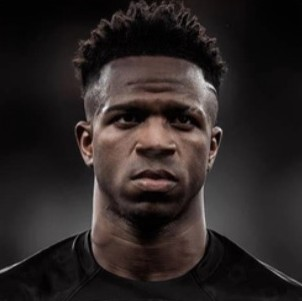
\includegraphics[width=0.5\textwidth]{img/b6.jpeg}
    \caption{Raw Generator Output}
\end{figure}

\section{Reconstructed Output}
\label{app:C7}
\begin{figure}[H]
    \centering
    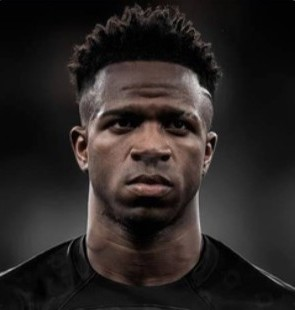
\includegraphics[width=0.5\textwidth]{img/b7.jpeg}
    \caption{Reconstructed Output}
\end{figure}


% ================= Appendix D =================
\chapter{User Interface Screenshots}
\label{app:D1}

\section{Main Interface}
\begin{figure}[H]
    \centering
    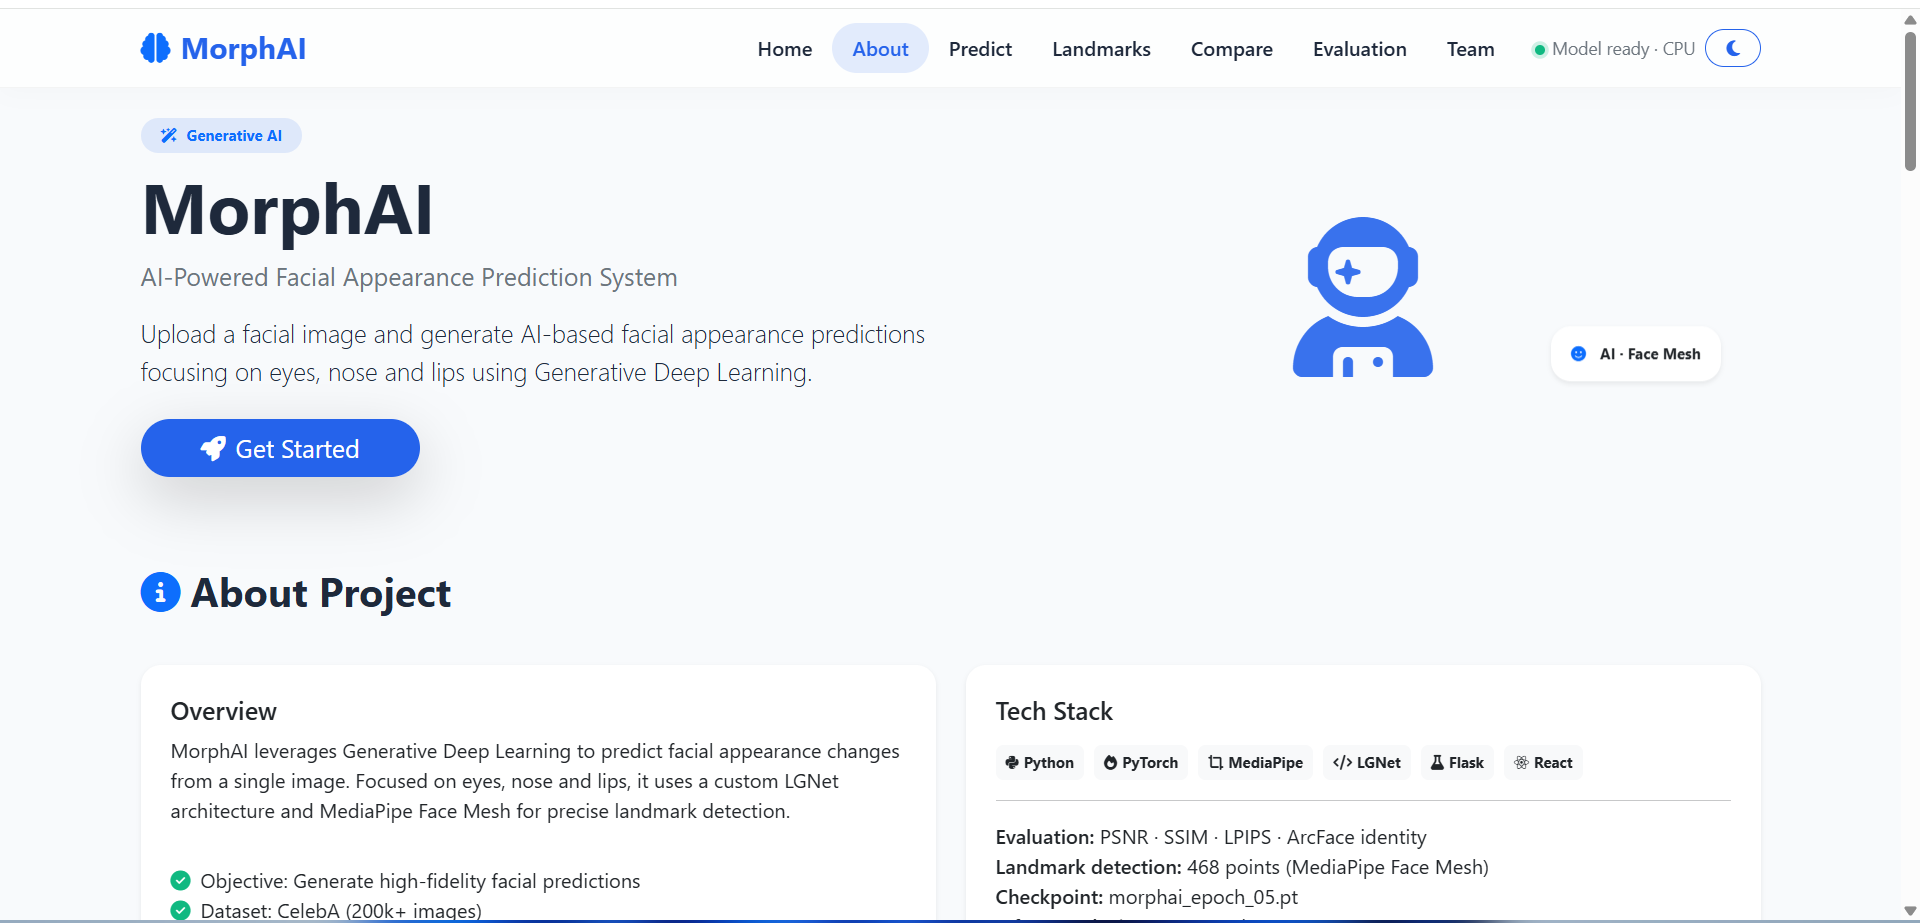
\includegraphics[width=0.72\textwidth]{img/UI.png}
    \caption{Main interface}
\end{figure}

\section{Input Image}
\begin{figure}[H]
    \centering
    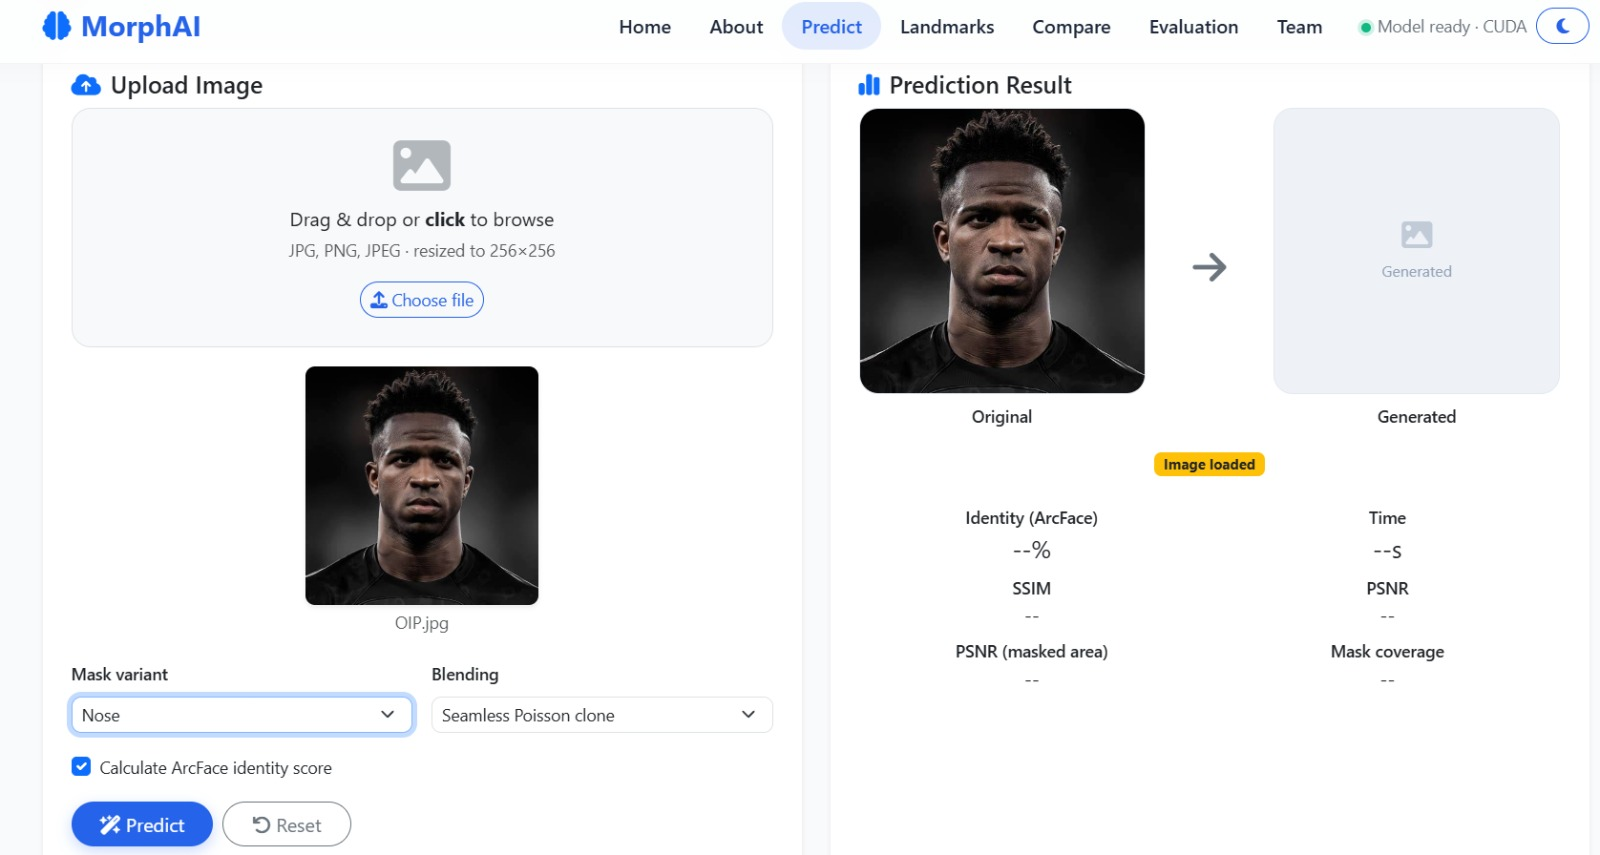
\includegraphics[width=0.75\textwidth]{img/c1.jpeg}
    \caption{Input Image}
\end{figure}

\section{Facial Landmark}
\begin{figure}[H]
    \centering
    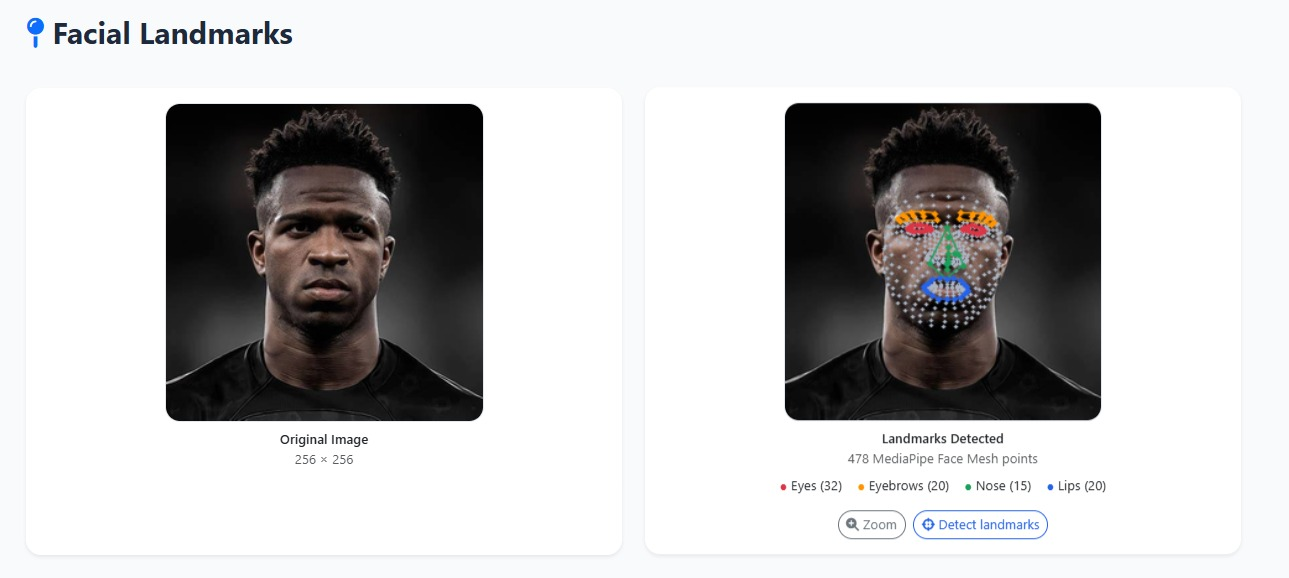
\includegraphics[width=0.75\textwidth]{img/c2.jpeg}
    \caption{Facial Landmark}
\end{figure}

\section{Inference Pipeline}
\begin{figure}[H]
    \centering
    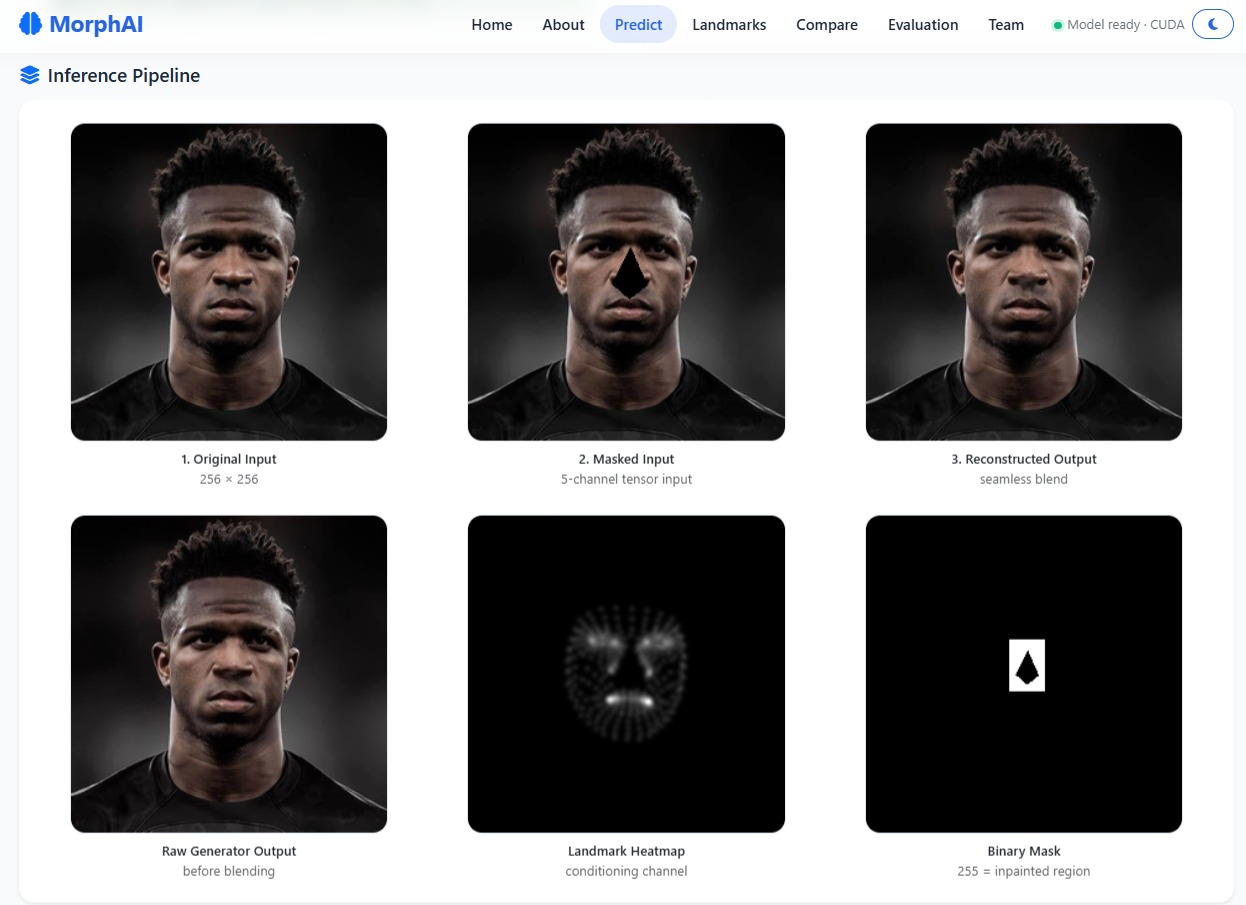
\includegraphics[width=0.75\textwidth]{img/c3.jpeg}
    \caption{Inference Pipeline}
\end{figure}

\section{Predicted Output}
\begin{figure}[H]
    \centering
    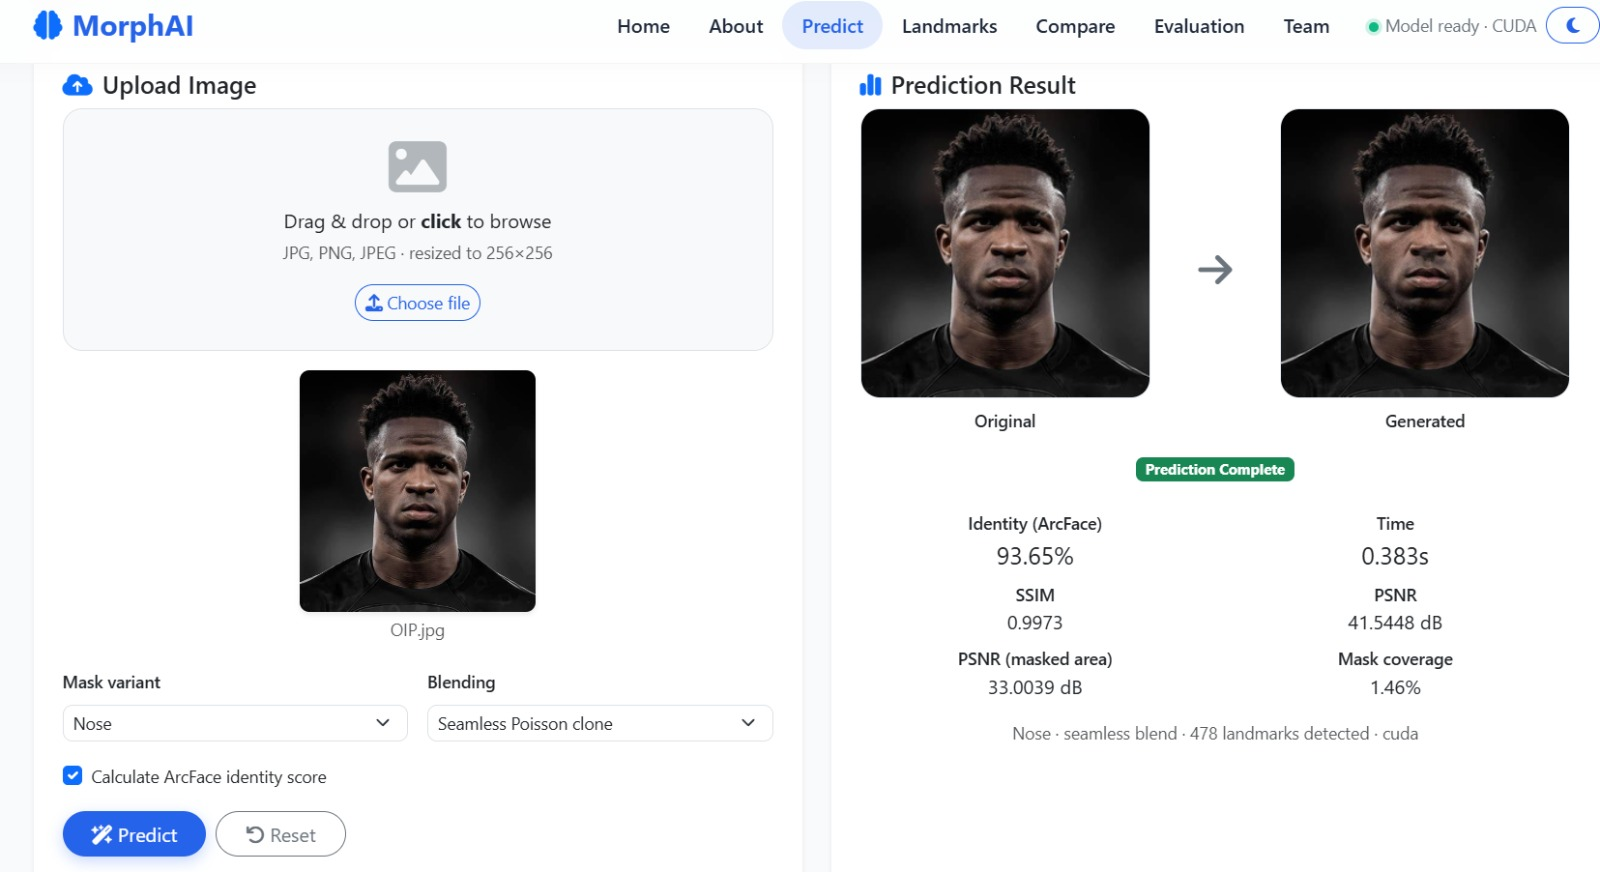
\includegraphics[width=0.75\textwidth]{img/c4.jpeg}
    \caption{Predicted Output}
\end{figure}